\section{Variational Autoencoders - VAEs}
\label{VAEs}

Based on the seminal work by \citeauthor{diggleImplicitPrescribed}, generative models can be classified into two broad categories. Prescribed models employ a well-defined, often parametric, mathematical expression for the probability density function (pdf), which enables easier analytical interpretation of the distributions. In contrast, implicit models synthesize new data samples without relying on an explicit pdf, approximating the underlying data distribution on which they were trained \citep{diggleImplicitPrescribed}. Variational Autoencoders (VAEs), which inherit the foundational architecture of autoencoders, belong to the prescribed models category as they require an explicit formulation of the probability density function (pdf) to function effectively. This feature makes VAEs suitable for tasks that require not only the generation but also the understanding of complex data distributions. \citep{kingmaVAE,rezendeVAE,GoodfellowDeepLearning}. Generative Adversarial Networks (GANs) \citep{goodfellowGAN}, discussed later, are a prime example ofthe latter category.

VAEs are essentially based on the architecture of autoencoders, which consist of an encoder and a decoder. The encoder aims to transform the input data into a low-dimensional latent space representation, commonly referred to as a "code" or "bottleneck" \citep{hintonCode, GoodfellowDeepLearning}. This code captures the most relevant features of the input while reducing its dimensionality. Then, the decoder attempts to reconstruct the original input from the obtained latent vector using a loss function. As explained by Goodfellow et al, an autoencoder that only succeeds in copying the exact representation of the input data does not itself prove useful. The essence of autoencoders lies in their ability to copy approximately rather than perfectly, which forces the model to prioritize which aspects of the input to copy \citep{GoodfellowDeepLearning}. This strategic approach often directs autoencoders to "learns useful properties of the data" \citep{GoodfellowDeepLearning}. To summarize, he main goal of an autoencoder is not the reconstruction itself, but the extraction of a meaningful latent vector that serves as a simplified representation of the input data.

The ability to reduce dimensionality has practical implications for improving the efficiency of classification tasks by reducing computational and memory overhead \citep{GoodfellowDeepLearning}. When paired with information retrieval, this dimensionality reduction makes searching in certain low-dimensional spaces particularly efficient \citep{GoodfellowDeepLearning}. Despite these advantages, traditional autoencoders are not designed to generate new data; their main function is to copy and reconstruct the given input \citep{GoodfellowDeepLearning}.

\begin{figure}[ht]
    \centering
      \hspace{.8cm}
      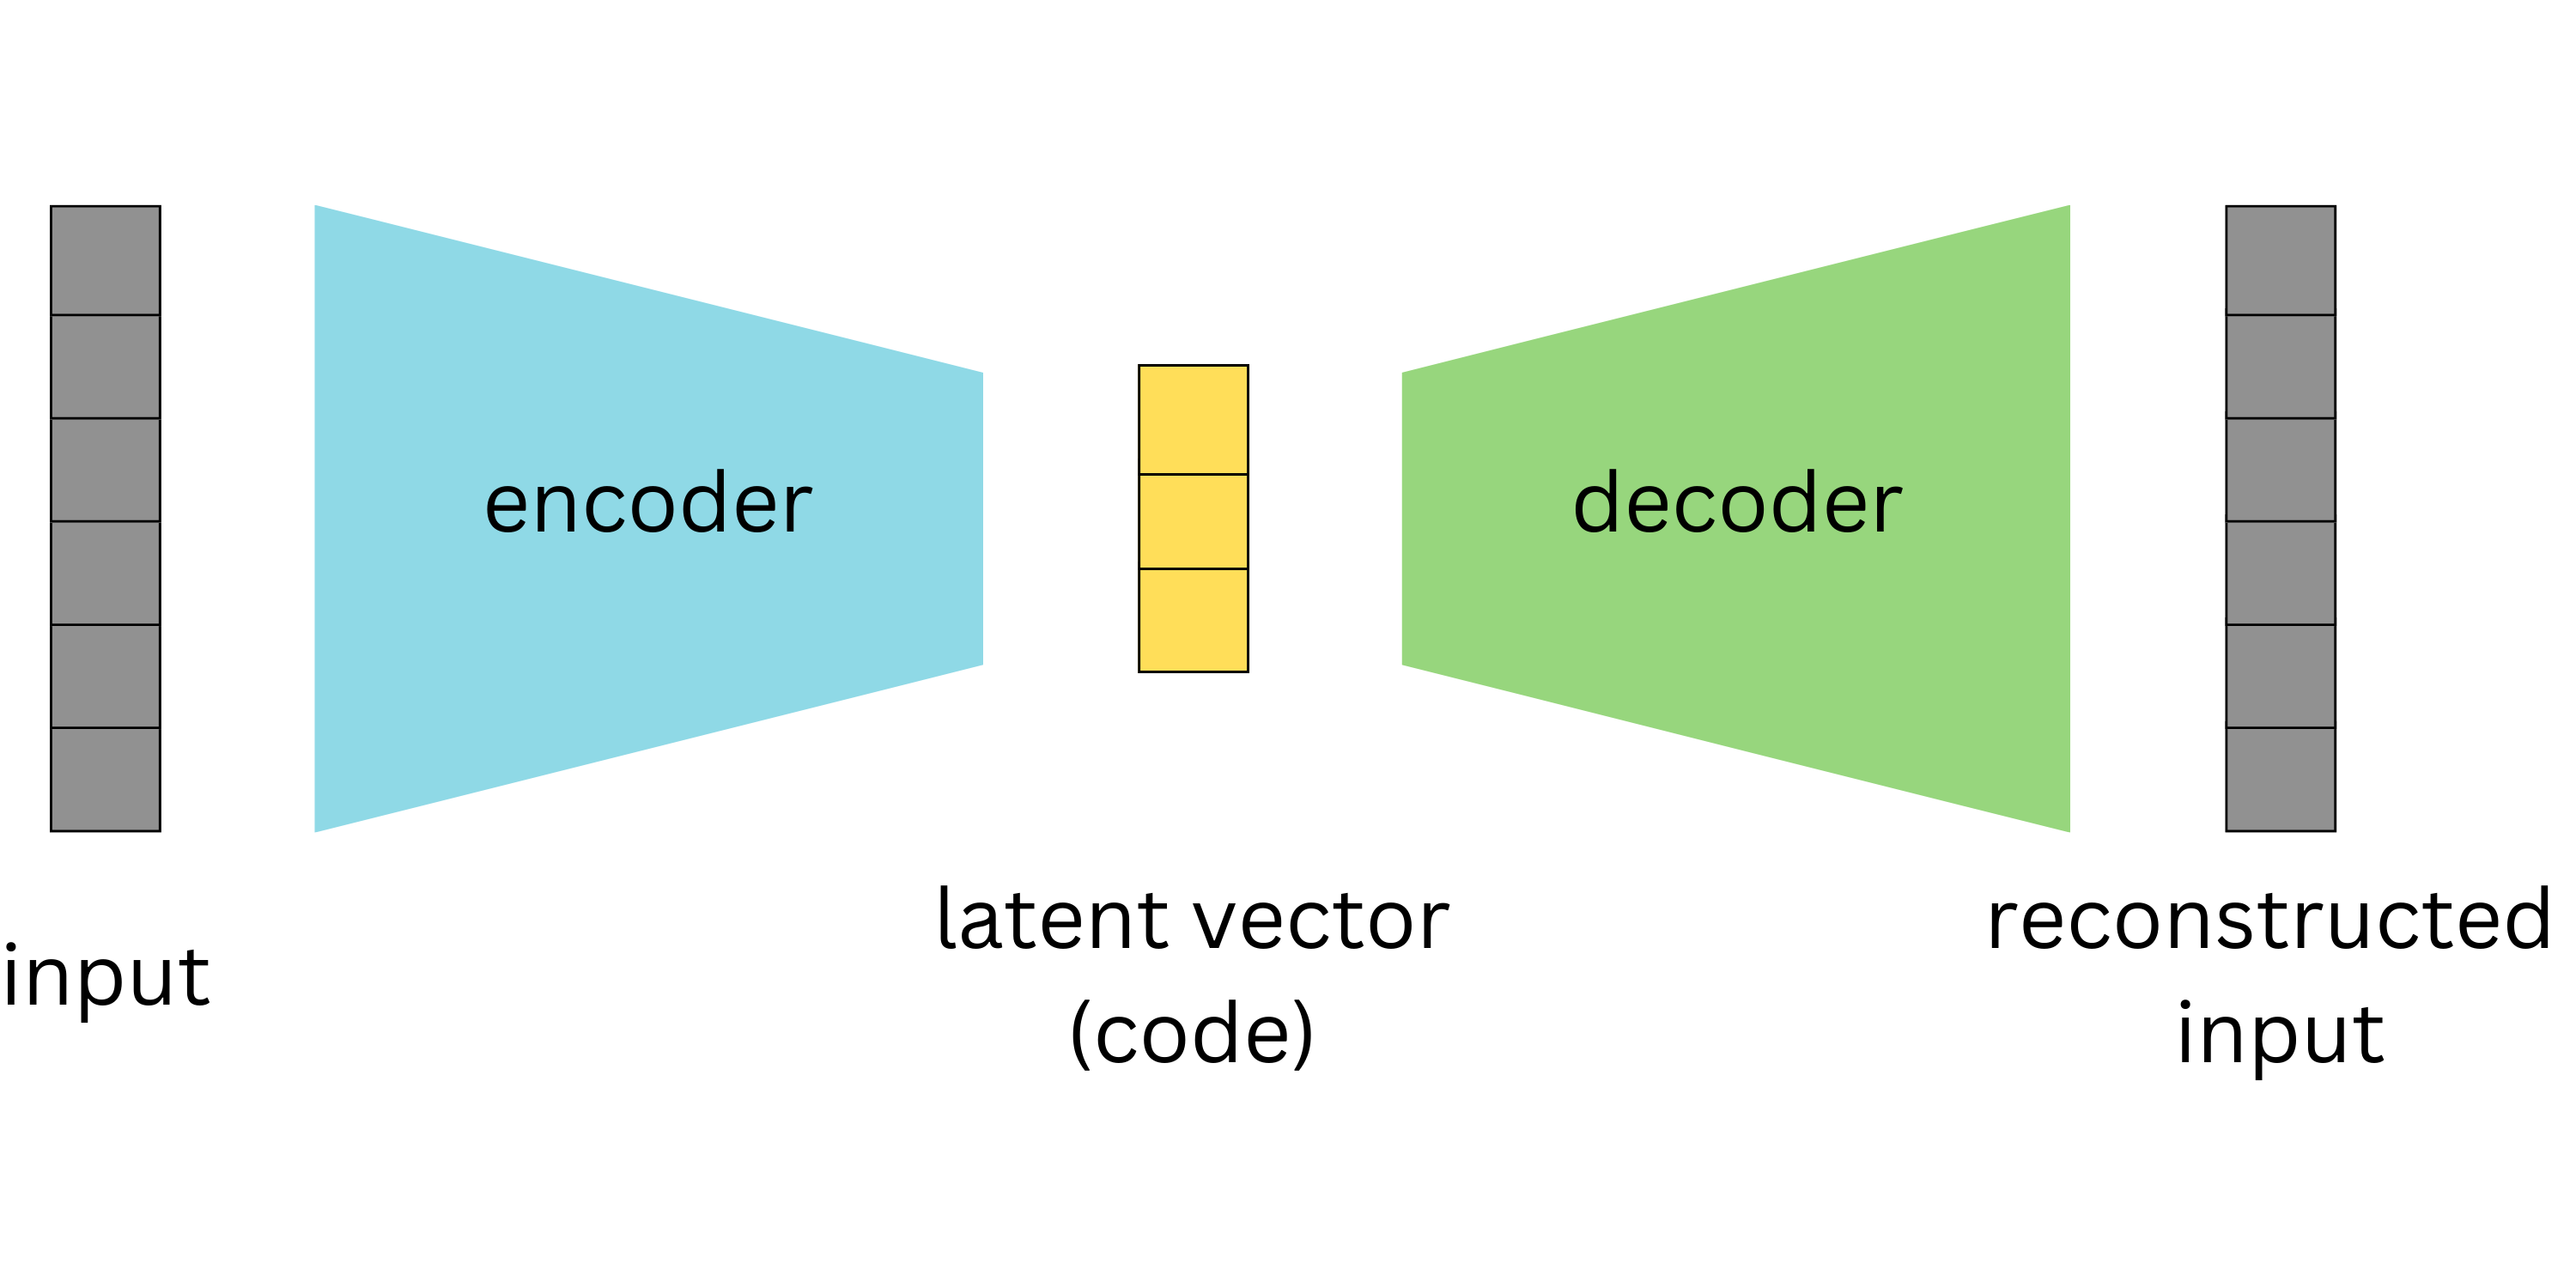
\includegraphics[width=.7\columnwidth]{figures/Autoencoder.png}
      \caption{Autoencoder: The encoder reduces the input dimension to a latent vector that captures the most important features. The decoder then uses this vector to reconstruct the input, with training aimed at minimizing reconstruction loss.}
      \label{fig:figureAE}
    \end{figure}


In variational autoencoders (VAEs), the encoder compresses the input into a space of latent variables and forms a probability distribution over these latent variables called \( q(z|x) \). This distribution helps with robustness against overfitting and enables the model to synthesize new analog data points. During the training phase, VAEs recognize specific regions in the latent variable space, similar to "pools," for different categories of data, allowing for a structured approach to data representation. Unlike standard autoencoders, where it is unclear where a useful latent vector can be sampled for the decoder, VAEs overcome this problem by restricting the latent space to known regions from which vectors can be safely sampled, as cited in \citep{doerschVAE}.

The procedure begins by selecting a sample \( z \) from a code distribution defined by the model, denoted \( p_{model}(z) \). This sample \( z \) is then passed through a differentiable generator network \( g(z) \). A sample \( x \) is then drawn from the distribution \( p_{model}(x; g(z)) \), where its properties are shaped by the processed \( z \) \citep{GoodfellowDeepLearning}. During the training phase, an approximate inference network, also called an encoder \( q(z|x) \), is used to infer \( z \) from \( x \), while \( p_{model}(x|z) \) works as a decoder network to reconstruct \( x \) from \( z \) \citep{GoodfellowDeepLearning}. The main training objective is embodied in the formula:
        
\begin{align}
  L(q) &= \mathbb{E}_{z \sim q(z|x)} \log p_{model}(z, x) + H(q(z|x)) \\
  &= \mathbb{E}_{z \sim q(z|x)} \log p_{model}(x|z) - D_{KL}(q(z|x) || p_{model}(z)) \\
  &\leq \log p_{model}(x)
\end{align}
        
Here, \( L(q) \) acts as a scorecard to evaluate the performance of UAE. The first term \( \log p_{\text{model}}(x|z) \) evaluates how well the UAE can fill in the details to recover the original input, while the second term \( D_{\text{KL}}(q(z|x) || p_{\text{model}}(z)) \) evaluates the complexity of the VAE representation compared to the original term, aiming for simplicity, as mentioned in \citep{GoodfellowDeepLearning}. 
        
The decoder in VAEs either reconstructs the original input or synthesizes new outputs from sampled latent variables. This process is optimized by a loss function that includes both the reconstruction loss and a regularization term based on the Kullback-Leibler (KL) divergence \( D_{\text{KL}} \). This divergence measures the discrepancies between the estimated and true data distributions \citep{kingmaVAE} and improves the model's ability to effectively generalize to unseen data.
        
Through this mechanism, VAEs continuously refine their representation and reconstruction process, improving the generation of new data points that resemble the original training data while maintaining a simplified and structured latent space.

\begin{figure}[ht]
    \centering
      \hspace{.8cm}
      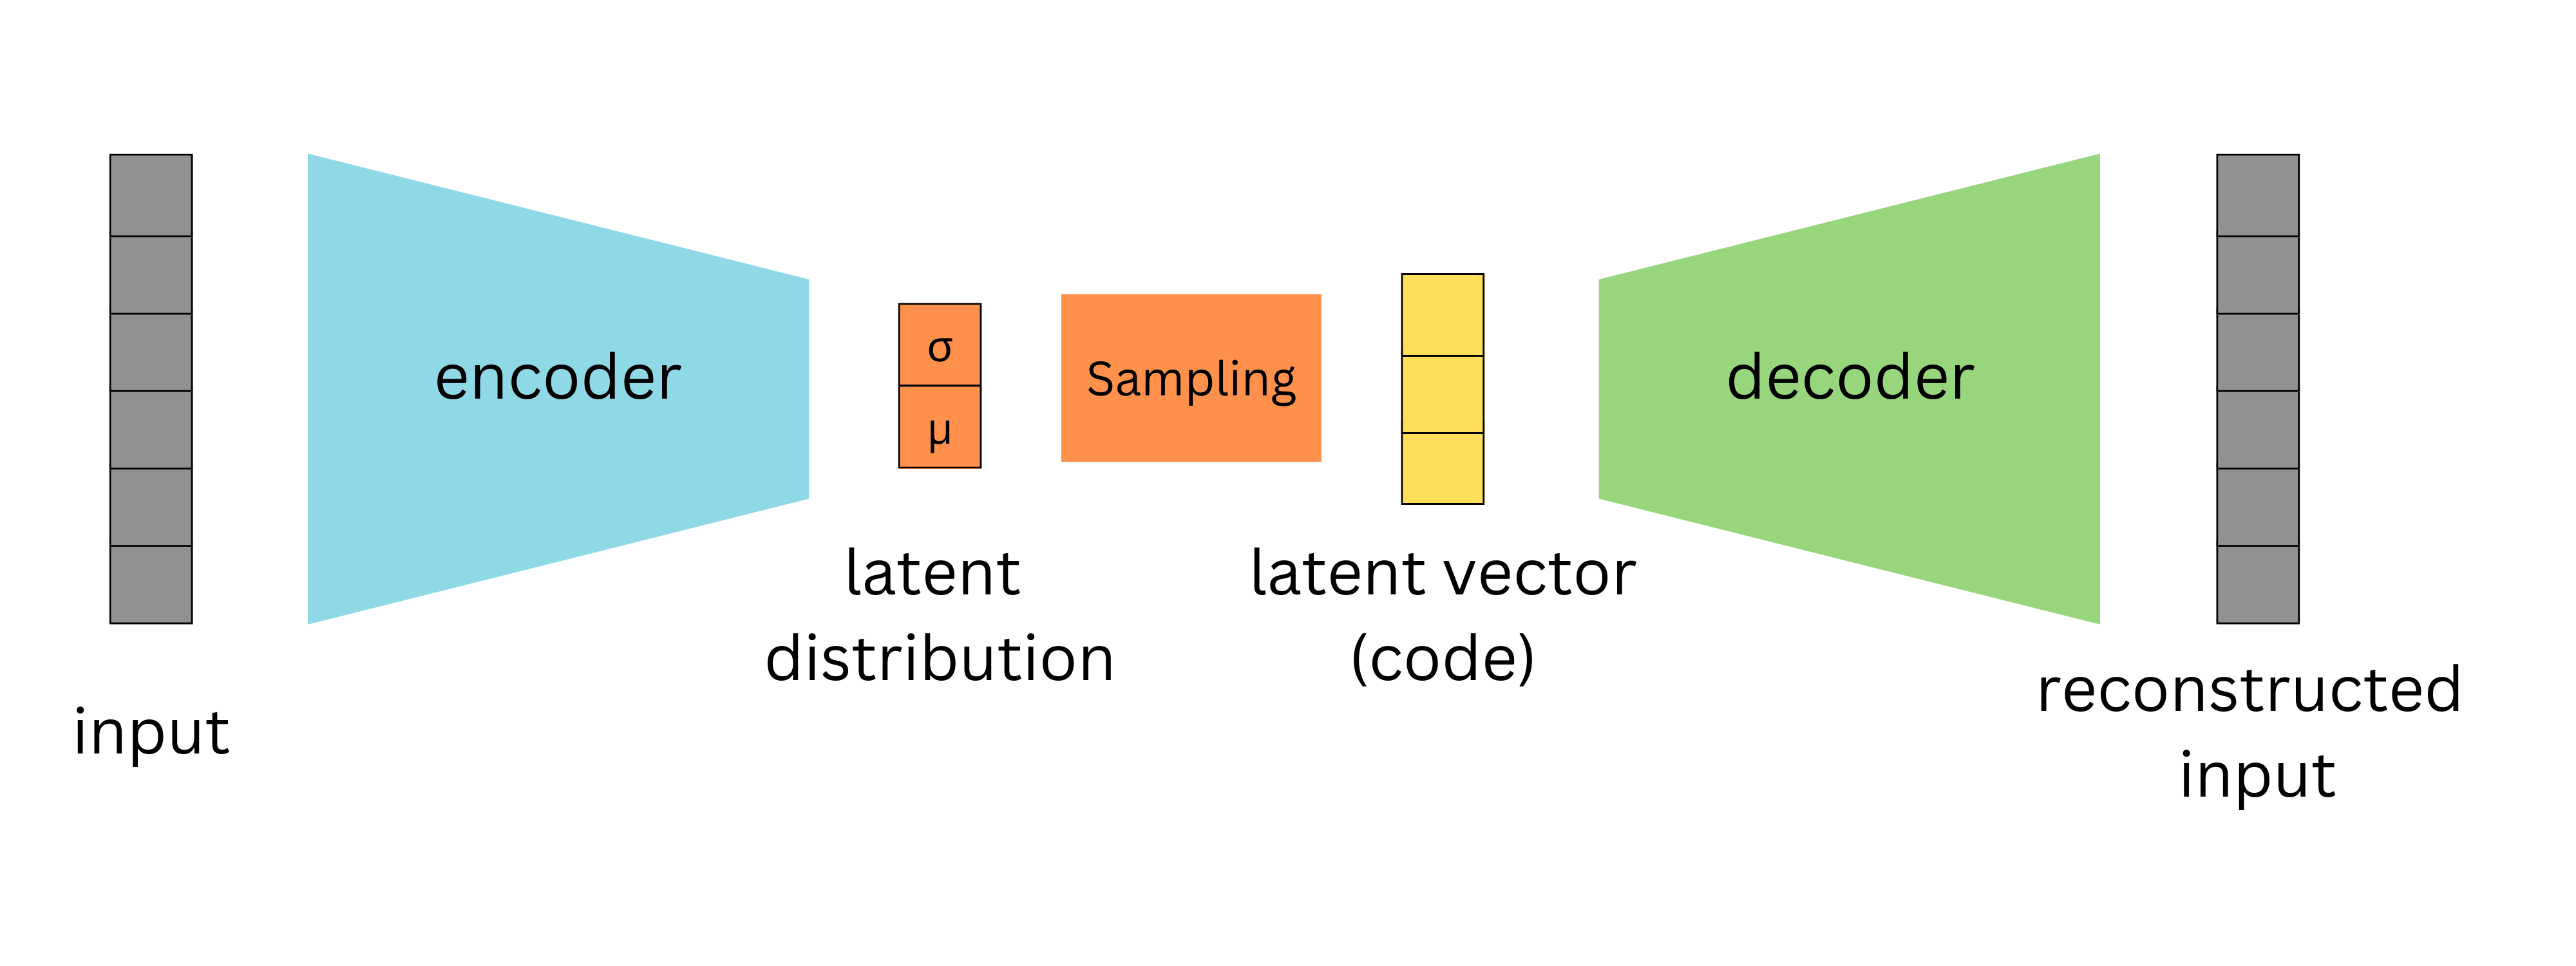
\includegraphics[width=.9\columnwidth]{figures/VAE.png}
      \caption{Functionality of a Variational Autoencoder, demonstrating incorporation of the latent distribution - the mean and standard deviation - for enhancing generative capabilities.}
      \label{fig:figureVAE}
\end{figure}

Despite their capabilities, VAEs exhibit some limitations. According to \citeauthor{GoodfellowDeepLearning}, the generated samples can often be blurry. The reason for this is not fully 
understood, but the blurriness observed may be due to their optimization process, which minimizes Kullback-Leibler divergence. This could lead the model to assign high probabilities to "points that occur in the training set, but may also assign high probability to other points [...] which may include blurry images" \citep{GoodfellowDeepLearning}. The Gaussian distribution often used in VAEs for the generative model may also contribute to this effect, as it can ignore minor features in the input data \citep{GoodfellowDeepLearning}. Another issue is that VAEs typically utilize only a small portion of the latent space, which might further compromise the quality of generated images \citep{GoodfellowDeepLearning}. The performance of the model is also sensitive to the choice of priors for the latent space, making hyperparameter tuning an essential aspect of working with VAEs \citep{kingmaVAE, higginsVAE}. 

